\documentclass{article}
\usepackage[landscape, margin=0.3in, top=0.5in, headheight=28pt, headsep=4pt]{geometry}
\usepackage{multicol}
\usepackage{tikz} 
\usetikzlibrary{decorations.pathmorphing}
\usetikzlibrary{fit}
\usepackage{xcolor}
\usepackage{fancyhdr}
\usepackage{enumitem}
\usepackage{fontspec}
\usepackage{titlesec}
\usepackage{amsmath}
\usepackage{graphicx}
\usepackage{svg}
\usepackage{float}
\usepackage{ifthen}
\usepackage{multirow}
\usepackage{colortbl}
\usepackage{caption}


\setmainfont[BoldFont={Montserrat-Medium}]{Montserrat-Regular}
\renewcommand{\baselinestretch}{0.9}
\renewcommand{\normalsize}{\fontsize{8}{8}\selectfont}

% Ensure the header/footer applies throughout
\thispagestyle{fancy}

% TikZ styles
\tikzstyle{mybox} = [draw=black, fill=white, very thick,
    rectangle, rounded corners, inner sep=5pt, inner ysep=14pt, minimum height=5cm, text centered, anchor=north]

\tikzstyle{fancytitle} = [
    draw=black,
    fill=black,
    very thick,
    rectangle, 
    rounded corners, 
    inner sep=4pt, 
    font=\bfseries\fontsize{10}{20}\selectfont\color{white}
]

\tikzstyle{fancytitleNull} = [draw opacity=0, fill opacity=0, very thick, rectangle, rounded corners, inner sep=4pt, font=\bfseries\fontsize{10}{20}\selectfont]

% Command definition for reusable fancybox
\newcommand{\fancybox}[2]{%
    \begin{tikzpicture}
        \node [mybox] (box) {%
            \begin{minipage}{0.9\linewidth} % Consistent width
            #2
            \end{minipage}
        };
        
               \ifthenelse{\equal{#1}{}}{%
            % If title is empty
            \node[fancytitleNull, right=10pt] at (box.north west) {NULL};
        }{%
            % If title is not empty
            \node[fancytitle, right=10pt] at (box.north west) {#1};
        }      
    \end{tikzpicture}%
}

% Global adjustments for section headings
\titleformat{\section}[hang]{\small\bfseries}{\thesection}{1em}{}
\titlespacing*{\section}{0pt}{-3pt}{0.5pt}

% Global adjustments for itemize lists
\let\olditemize\itemize
\def\itemize{\olditemize
  \renewcommand{\labelitemi}{\fontsize{8}{16}\selectfont$\bullet$}
}
\setlist[itemize]{left=6pt, itemsep=3pt, parsep=0pt, partopsep=0pt}
\setlist[enumerate]{left=6pt, itemsep=3pt, parsep=0pt, partopsep=0pt}

% Header settings
\pagestyle{fancy} % Enable fancy header and footer
\fancyhf{} % Clear default header and footer
\chead{\fontsize{14}{18}\selectfont \textbf{ISTQB - Certified Tester Foundation Level (CTFL) v4.0}}
\renewcommand{\headrulewidth}{0pt}
\rhead{\thepage}


% Footer customization
\cfoot{\textbf{Antonia Frey} \ \textperiodcentered\  \the\day-\the\month-\the\year} 
\renewcommand{\footrulewidth}{0pt} 
\setlength{\footskip}{0in} 




\begin{document}

%\begin{center}
%    {\large{\textbf{}}}
%\end{center}

\noindent
\begin{multicols}{3}

%------------ 1. Fundamentals of Testing ---------------
\fancybox{1. Fundamentals of Testing}{

\section*{What is Testing?}
Software testing is a set of activities to discover defects and evaluate the quality of software work products.

\section*{Why is Testing Necessary?}
Testing, as a form of quality control, helps in achieving the agreed upon test objectives within the set scope, time, quality, and budget constraints.\\

\section*{Testing and Debugging}
\begin{itemize}
\item \textbf{Testing} can trigger failures that are caused by defects in the software (dynamic testing) or can directly find defects in the test object (static testing)
\item \textbf{Debugging} is concerned with finding causes of this failure (defects), analyzing and eliminating them. 
\end{itemize}

\section*{Testing and Quality Assurance}
\begin{itemize}
  \item Testing is product-oriented
  \item QA is process-oriented
\end{itemize}

\section*{Errors, Defects, Failues, and Root Causes}
Human beings make errors (mistakes), which produce defects (faults, bugs), which may result in failures. Failures can also be caused by environmental conditions.\\

\section*{Testing Principles}
\begin{enumerate}
  \item Testing shows the presence of defects. 
  \item Exhaustive testing is impossible. 
  \item Early testing saves time and money. 
  \item Defects cluster together.
  \item Tests wear out.
  \item Testing is context dependent. 
  \item Absence-of-defects fallacy.
\end{enumerate}

\section*{Test Activities and Tasks}
\begin{itemize}
  \item Test planning
  \item Test monitoring and test control
  \item Test analysis
  \item Test design
  \item Test implementation
  \item Test execution
  \item Test completion
\end{itemize}

\section*{Roles in Testing}
\begin{itemize}
  \item \textbf{Test Management Role:} Takes overall responsibility for the test process, test team and leadership of the test activities.
  \item \textbf{Testing Role:} Focused on the activities of test analysis, test design, test implementation and execution.
\end{itemize}

\section*{Good Practices}
\begin{itemize}
    \item \textbf{Whole Team Approach:}
    Any team member can perform any task, everyone is responsible for quality.
    
    \item \textbf{Independence of Testing:}
    Independent testers recognize different kinds of failures and defects, but may be isolated from the development team, causing poor collaboration.
\end{itemize}
}

%------------ 2. Testing Throughout the SDLC ---------------
\fancybox{2. Testing Throughout the SDLC}{
\section*{Software Development Lifecycle (SDLC)}
An SDLC model is an abstract, high-level representation of the software development process. Every software development activity has a corresponding test activity.\\


\section*{Testing as a Driver for Software Development}
\begin{itemize}
  \item \textbf{Test-Driven Development (TDD)}\\
  Tests are written first, then the code is written to satisfy the tests.
  \item \textbf{Acceptance Test-Driven Development (ATDD)}\\
  Tests are derived from acceptance criteria and written before development of the application part. 
  \item \textbf{Behavior-Driven Development (BDD)}\\
  Tests are written in simple natural language (e.g., Given/When/Then) to express desired behavior.
\end{itemize}

\section*{Shift Left}
The principle of early testing is sometimes referred to as shift left because it is an approach where testing is performed earlier in the SDLC.\\

\section*{Test Levels}
Test levels are groups of test activities that are organized and managed together. There are five test levels:
\begin{itemize}
  \item \textbf{Component testing (unit testing)}\\
  Testing components in isolation.
  
  \item \textbf{Component integration testing}\\
  Testing interactions between components.
  
  \item \textbf{System testing}\\
  Testing the overall behavior and capabilities of an entire system or product, including functional and non-functional testing.
  
  \item \textbf{System integration testing}\\
  Testing interfaces of the system under test and other systems and external services.
  
  \item \textbf{Acceptance testing}\\
  Focuses on validation and on demonstrating readiness for deployment, which means that the system fulfills the user’s business needs.
\end{itemize}

\section*{Test Types}
\begin{itemize}
  \item \textbf{Functional testing} evaluates the functions that a component or system should perform. The functions are “what” the test object should do.
  \item \textbf{Non-functional testing} is the testing of “how well the system behaves”. These include aspects such as performance efficiency, compatibility, and usability.
  \item \textbf{Black-box testing} is specification-based.
  \item \textbf{White-box testing} is structure-based.
\end{itemize}

\section*{Maintenance Testing}
\begin{itemize}
  \item \textbf{Confirmation Testing} confirms that an original defect has been fixed.
  \item \textbf{Regression Testing} confirms that no adverse consequences have been caused by a change.
\end{itemize}
}

%------------ 3. Static Testing ---------------
\fancybox{3. Static Testing}{
\section*{Static Testing Basics}
In contrast to dynamic testing, in static testing the software under test does not need to be executed. Static analysis can identify problems prior to dynamic testing while often requiring less effort, since no test cases are required, and tools are typically used.\\

\section*{Static Testing vs. Dynamic Testing}
\begin{itemize}
\item Some defect types that can only be found by either static or dynamic testing.
\item Static testing finds defects directly, while dynamic testing causes failures.
\item Static testing may more easily detect defects that lay on paths through the code that are rarely executed.
\item Static testing can be applied to non-executable work products.
\end{itemize}

\section*{Stakeholder Feedback}
Early and frequent feedback allows for the early communication of potential quality problems.\\

\section*{Review Process Activities}
\begin{itemize}
    \item Planning
    \item Review Initiation
    \item Individual Review
    \item Communication and Analysis
    \item Fixing and Reporting
\end{itemize}
\section*{Roles and Responsibilities in Reviews}
\begin{itemize}
    \item Manager – decides what to review and provides resources
    \item Author – creates and fixes the work product
    \item Moderator (also known as the facilitator) – runs review meetings and ensures a safe environment
    \item Scribe (also known as recorder) – records anomalies and decisions during the review
    \item Reviewer – performs the review, may be a subject expert or stakeholder
    \item Review leader – takes overall responsibility for review
\end{itemize}

\section*{Review Types}
\begin{itemize}
    \item Informal review – does not follow a defined process and does not require formal documented output.
    \item Walkthrough – led by the author, used for evaluating quality, building confidence, educating reviewers, and detecting anomalies.
    \item Technical Review – performed by technically qualified reviewers, led by a moderator. The goal is to make decisions regarding technical problems and detect anomalies.
    \item Inspection – the most formal type of review, following the complete generic process. The main objective is to find the maximum number of anomalies, evaluate quality, and improve the SDLC.
\end{itemize}
}

%------------ 4. Test Analysis and Design ---------------
\fancybox{4. Test Analysis and Design}{

\section*{Test Techniques}
\begin{itemize}

\item \textbf{Black-box Test Techniques (specification-based)}\\
Analysis of the specified behavior of the test object without reference to its internal structure. Therefore, the test cases are independent of how the software is implemented.

\begin{itemize}
    \item Equivalence Partitioning
    \item Boundary Value Analysis
    \item Decision Table Testing
    \item State Transition Testing
\end{itemize}

\item \textbf{White-box Test Techniques (structure-based)}\\
Analysis of the test object’s internal structure and processing. As the test cases are dependent on how the software is designed, they can only be created after the design or implementation of the test object.

\begin{itemize}
    \item Statement testing
    \item Branch testing
\end{itemize}

\item \textbf{Experience-based Test Techniques}\\
Use the knowledge and experience of testers for the design and implementation of test cases. These test techniques depends on the tester’s skills.

\begin{itemize}
    \item Error guessing
    \item Exploratory testing
    \item Checklist-based testing
\end{itemize}

\end{itemize}

\section*{Collaborative User Story Writing}
A user story represents a feature that will be valuable to either a user or purchaser of a system or software. User stories have three critical aspects, called the “3 C’s”:

\begin{itemize}
    \item \textbf{Card} – the medium describing a user story (e.g., an index card, an entry in an electronic board)
    \item \textbf{Conversation} – explains how the software will be used (can be documented or verbal)
    \item \textbf{Confirmation} – the acceptance criteria
\end{itemize}
The most common format for a user story is “As a [role], I want [goal to be accomplished], so that I can [resulting business value for the role]”, followed by the acceptance criteria.\\

\section*{Acceptance Criteria}
Acceptance criteria for a user story are the conditions that an implementation of the user story must meet to be accepted by stakeholders.\\

\section*{Acceptance Test-driven Development}
ATDD is a test-first approach. Test cases are created prior to implementing the user story. The test cases are based on the acceptance criteria and can be seen as examples of how the software works. Examples and tests are the same.
}

%------------ 5. Managing the Test Activities ---------------
\fancybox{5. Managing the Test Activities}{
\section*{Test Plan}
A test plan describes the test objectives, resources and processes for a test project.\\

\section*{Entry Criteria and Exit Criteria}
Entry criteria define the preconditions for undertaking a given activity. Exit criteria define what must be achieved to declare an activity completed. Entry criteria and exit criteria should be defined for each test level, and will differ based on the test objectives.\\

\section*{Estimation Techniques}
\begin{itemize}
    \item \textbf{Estimation Based on Ratios}
    \item \textbf{Extrapolation}
    \item \textbf{Wideband Delphi} (e.g. Planning Poker)
     \begin{itemize}
        \item Commonly used in Agile SW development 
    \end{itemize}
    \item \textbf{Three-Point Estimation}\\
\vspace{-20pt}  
\begin{figure}[H]
  \begin{minipage}{0.5\textwidth}
  \text{Estimate:}\\
    \begin{equation*}
      E = \frac{a + 4m + b}{6} \quad \text{where:}
    \end{equation*}
    
  \end{minipage}
  \begin{minipage}{0.3\textwidth}
    \begin{flalign*}
      a & = \text{optimistic estimate} \\
      m & = \text{most likely estimate} \\
      b & = \text{pessimistic estimate}
    \end{flalign*}
  \end{minipage}
\end{figure}

\vspace{-20pt}  
\begin{figure}[H]
  \begin{minipage}{0.3\textwidth}
  \text{Measurement error:}\\
\begin{equation*}
SD = \frac{b - a}{6}
\end{equation*}
    
  \end{minipage}
  \begin{minipage}{0.7\textwidth}
  \end{minipage}
\end{figure}
 
\end{itemize}

\section*{Test Case Prioritization}
When prioritizing test cases, different factors can be taken into account. The most commonly used test case prioritization strategies are as follows:
\begin{itemize}
    \item \textbf{Risk-based prioritization}\\
    Test cases covering the most important risks are executed first.
    
    \item \textbf{Coverage-based prioritization}\\
    Test cases achieving the highest coverage are executed first.
    
    \item \textbf{Requirements-based prioritization}\\
    Test cases related to the most important requirements are executed first.
\end{itemize}

\section*{Test Pyramid}
 Tests in the bottom layer are small, isolated, fast, and check small pieces of functionality, a lot of them are needed for coverage. The top layer represents complex, high-level, end-to-end tests.
\begin{figure}[H]
  \begin{minipage}{0.45\textwidth}
    \centering
    \includesvg[width=\textwidth]{pyramid.svg}
  \end{minipage}%
  \hspace{0.05\textwidth} % Adjust space between image and text
  \begin{minipage}{0.5\textwidth}
  \raggedright % Left align the content
\begin{itemize}
\item UI tests,\\ end-to-end (E2E) tests 
\item Service tests,\\ Integration test
\item Unit tests,\\ Component tests
\end{itemize}
  \end{minipage}
\end{figure}

}

\fancybox{}{
\vspace{-10pt}
\section*{Testing Quadrants}
The testing quadrants, defined by Brian Marick (Marick 2003, Crispin 2008), group the test levels with the appropriate test types, activities, test techniques and work products in the Agile software development.
\vspace{-10pt}
\begin{figure}[H]
    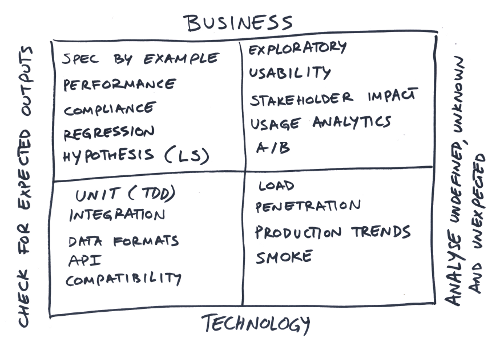
\includegraphics[width=0.8\textwidth]{quadrants.png}
    \vspace{-10pt}
\end{figure}


\begin{itemize}
  \item \textbf{Quadrant Q1} (technology facing, support the team): This quadrant contains component tests and component integration tests. These tests should be automated and included in the CI process.
  \item \textbf{Quadrant Q2} (business facing, support the team): This quadrant contains functional tests, examples, user story tests, user experience prototypes, API testing, and simulations. These tests check the acceptance criteria and can be manual or automated.
  \item \textbf{Quadrant Q3} (business facing, critique the product): This quadrant contains exploratory testing, usability testing, user acceptance testing. These tests are user-oriented and often manual.
  \item \textbf{Quadrant Q4} (technology facing, critique the product): This quadrant contains smoke tests and non-functional tests (except usability tests). These tests are often automated.
\end{itemize}

\section*{Risk Management}
The main risk management activities are:
\vspace{-5pt}
\begin{itemize}
  \item \textbf{Risk analysis}: Risk identification and -assessment
  \item \textbf{Risk control} Risk mitigation and -monitoring
\end{itemize}
A risk can be characterized by two factors:
\vspace{-5pt}
\begin{itemize}
\item Risk likelihood – probability of risk occurrence (0-1)
\item Risk impact (harm) – consequences of occurrence
\end{itemize}
In software testing there are two types of risks:
\vspace{-5pt}
\begin{itemize}
\item project risks - management issues
\item product risks - product quality characteristics
\end{itemize}

\section*{Configuration Management (CM)}
CM provides a discipline for identifying, controlling, and tracking work products such as test plans, test strategies, test conditions, test cases, test scripts, test results, test logs, and test reports as configuration items.

\section*{Defect Management}
Workflow for handling individual defects or anomalies from their discovery to their closure and rules for their classification.

}

%------------ 6. Test Tools ---------------
\fancybox{6. Test Tools}{
\section*{Tool Support for Testig}
\begin{itemize}
  \item \textbf{Test management tools}\\
  Tools to increase the test process efficiency by facilitating management of the SDLC, requirements, tests, defects, configuration
  
  \item \textbf{Static testing tools}\\
  Tools to support the tester in performing reviews and static analysis
  
  \item \textbf{Test design and test implementation tools}\\
  Tools to generate test cases, test data, and test procedures
  
  \item \textbf{Test execution and test coverage tools}\\
  Tools for automated test execution and coverage measurement
  
  \item \textbf{Non-functional testing tools}\\
  Tools to perform non-functional testing that is difficult or impossible to perform manually
  
  \item \textbf{DevOps tools}\\
  Tools to support the DevOps delivery pipeline, workflow tracking, automated build processes, CI/CD
  
  \item \textbf{Collaboration tools} – facilitate communication
  \item \textbf{Tools supporting scalability and deployment standardization} (e.g., VMs, containerization tools)
  \item \textbf{Other tools}\\
  (e.g., a spreadsheet is a tool in the context of testing)
\end{itemize}

\section*{Benefits and Risks of Test Automation}
Benefits of test automation:
\begin{itemize}
  \item Time saved by reducing repetitive manual work
  \item Prevention of simple human errors
  \item More objective assessment
  \item Access to information (e.g., statistics, failure rates)
  \item Reduced test execution time
\end{itemize}

Risks of test automation:
\begin{itemize}
  \item Unrealistic expectations
  \item Inaccurate estimations of time, costs, effort
  \item Using a test tool when manual testing is more appropriate
  \item Relying on a tool too much
  \item Dependency on tool vendor
  \item Problems with open-source software
  \item Incompatiblility of  tool with the development platform
  \item Choosing an unsuitable tool (Compliance and standards)
\end{itemize}
}


%------------ Certification ---------------
\fancybox{Certification}{

\section*{ISTQB}
The International Software Testing Qualifications Board (ISTQB) is a software testing certification board.\\

\section*{Overview}
The ISTQB Certified Tester Foundation Level (CTFL) certification is the cornerstone of essential testing knowledge that can be applied to real-world scenarios.\\

\section*{Exam Structure}
\begin{itemize}
    \item \textbf{No. of Questions}: 40
    \item \textbf{Passing Score}: 26
    \item \textbf{Total Points}: 40
    \item \textbf{Time (min)}: 60 (+15 min for Non-Native Language)
\end{itemize}

\section*{Learning objectives levels}
\begin{itemize}
\item K1: Remember
\item K2: Understand
\item K3: Apply
\end{itemize}

\section*{Exam Structures Rules}
\vspace{-10pt}
\begin{table}[H]
\renewcommand{\arraystretch}{2}
\centering
\begin{tabular}{|c|c|c|c|}
\hline
\rowcolor{black} \textcolor{white}{\textbf{K-Level}} & 
\textcolor{white}{\textbf{No. of Questions}} & 
\textcolor{white}{\textbf{Time}} & 
\textcolor{white}{\textbf{Total Time}} \\ \hline
K1                              & 8                                              & 1                                    & 8                       \\ \hline
K2                              & 24                                             & 1                                    & 24                      \\ \hline
K3                              & 8                                              & 3                                    & 24                      \\ \hline
\hline
\textbf{Total}                 & \textbf{40}                                    &                               & \textbf{56 min}             \\ \hline
\end{tabular}
\caption*{K-Level Breakdown and Total Time}
\end{table}

\begin{table}[H] 
\renewcommand{\arraystretch}{2}
\centering
\begin{tabular}{|c|c|c|c|c|c|}
\hline
\cellcolor{black}\textcolor{white}{\textbf{Chapter}} & \cellcolor{black}\textcolor{white}{\textbf{K1}} & \cellcolor{black}\textcolor{white}{\textbf{K2}} & \cellcolor{black}\textcolor{white}{\textbf{K3}} & \cellcolor{black}\textcolor{white}{\textbf{Points}} & \cellcolor{black}\textcolor{white}{\textbf{Percentage}} \\ \hline
\textbf{Chapter 1} & 2 & 6 & 0 & 8 & \textbf{13\%} \\ \hline
\textbf{Chapter 2} & 1 & 4 & 0 & 5 & \textbf{8\%} \\ \hline
\textbf{Chapter 3} & 1 & 3 & 1 & 5 & \textbf{8\%} \\ \hline
\textbf{Chapter 4} & 1 & 5 & 5 & 11 & \textbf{18\%} \\ \hline
\textbf{Chapter 5} & 2 & 5 & 2 & 9 & \textbf{15\%} \\ \hline
\textbf{Chapter 6} & 1 & 1 & 0 & 2 & \textbf{3\%} \\ \hline \hline
\textbf{Total} & 10 & 24 & 8 & 60 & 100\% \\ \hline
\end{tabular} 
\caption*{Question Breakdown by Chapter and K-Level}
\end{table}
}

\fancybox{Keywords (K1)}{
\section*{Overview}
All terms listed as keywords shall be remembered (K1), even if not explicitly mentioned in the learning objectives.\\

\section*{1. Fundamentals of Testing}
coverage, debugging, defect, error, failure, quality, quality assurance, root cause, test analysis, test basis, test case, test completion, test condition, test control, test data, test design, test execution, test implementation, test monitoring, test object, test objective, test planning, test procedure, test process, test result, testing, testware, traceability, validation, verification\\

\section*{2. Testing Throughout the SDLC}
acceptance testing, black-box testing, component integration testing, component testing, confirmation testing, functional testing, integration testing, maintenance testing, non-functional testing, regression testing, shift left, system integration testing, system testing, test level, test object, test type, white-box testing\\

\section*{3. Static Testing}
anomaly, dynamic testing, formal review, informal review, inspection, review, static analysis, static testing, technical review, walkthrough\\

\section*{4. Test Analysis and Design}
acceptance criteria, acceptance test-driven development, black-box test technique, boundary value analysis, branch coverage, checklist-based testing, collaboration-based test approach, coverage, coverage item, decision table testing, equivalence partitioning, error guessing, experience-based test technique, exploratory testing, state transition testing, statement coverage, test technique, white-box test technique\\

\section*{5. Managing the Test Activities}
defect management, defect report, entry criteria, exit criteria, product risk, project risk, risk, risk analysis, risk assessment, risk control, risk identification, risk level, risk management, risk mitigation, risk monitoring, risk-based testing, test approach, test completion report, test control, test monitoring, test plan, test planning, test progress report, test pyramid, test strategy, testing quadrants\\

\section*{6. Test Tools}
test automation
}





\end{multicols}

\end{document}
